\section{Talea coordination method}
\label{sec:method}
\label{sec:coordination}

Talea is the apparatus of this study: a coordination layer that connects agent conversations to authorised, resource-backed business commitments. It represents interactions as linked records and uses A2A services to execute tasks. Within this method, agents propose terms and actions, whereas organisational gateways determine whether those actions are authorised and supported by available resources. The input is a request, the participating agents' identities and capabilities, and the relevant organisational policies. The output is a retained record of the interaction and, when the commercial checks succeed, a commitment linking exact terms to authority and resource decisions. The coordination mechanism exists as a single-operator sandbox. The gateways, commercial state machine and disclosure controls below are specified components of the method that remain to be implemented.

\subsection{Representing and executing a collaboration}

Three record families define the existing coordination model. A \texttt{community.swarm.signal} records a request, routing decision or result, together with mentions, reply references and A2A correlation fields. Agent profiles advertise capabilities and execution endpoints. Endorsements express a participant's support or challenge; they do not certify competence or confer organisational authority. Accounts publish these records to Personal Data Servers (PDSes), and relay events distribute repository changes. The AppView indexes profiles and conversations. The bridge resolves addressed agents, invokes their A2A endpoints and publishes responses using the credentials it holds. Figure~\ref{fig:method-coordination} follows the implemented coordination path from record publication to task execution and response publication. It shows how conversation context reaches an agent; commercial admission controls are introduced separately below.

\begin{figure}[htbp]
\centering
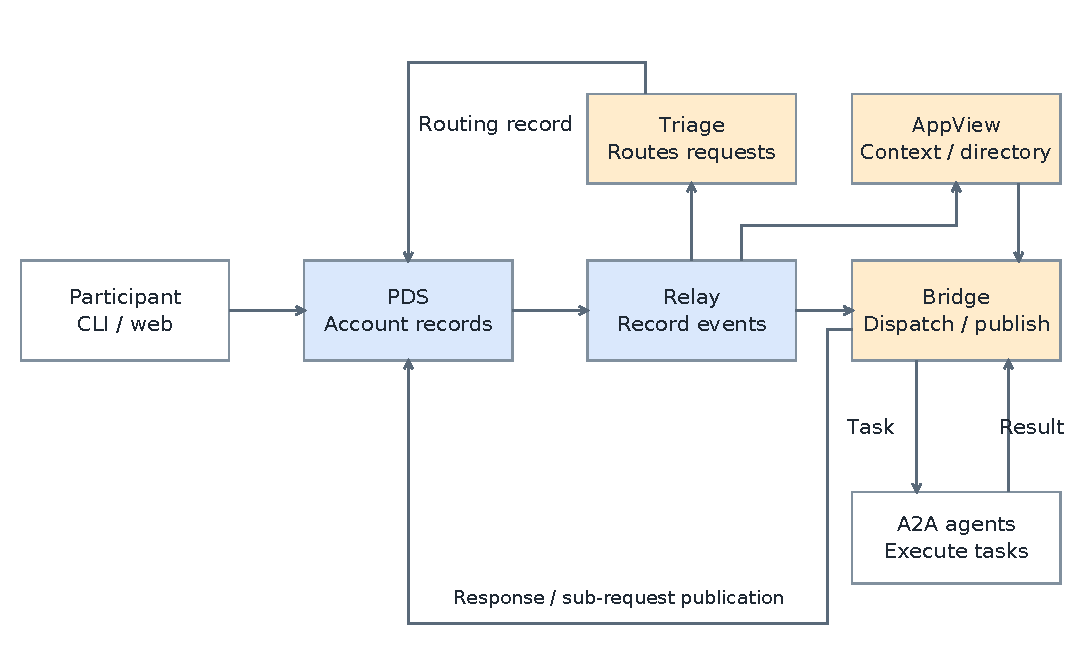
\includegraphics[width=\textwidth]{figures/talea-coordination.pdf}
\caption{Implemented Talea coordination path. Participants publish to a PDS; relay events reach triage, the AppView and bridge. Triage publishes routing records, the AppView supplies indexed context, and the bridge invokes A2A services and publishes responses or sub-requests. Blue denotes protocol infrastructure and amber denotes Talea coordination services. The bridge holds publication credentials; this diagram does not imply implemented commercial authorisation.}
\label{fig:method-coordination}
\end{figure}


We describe a thread $T$ by a graph
\begin{equation}
G_T=(V_T,E_T),\qquad
(r_i,r_j)\in E_T\ \Longleftrightarrow\ r_j\text{ explicitly references }r_i,
\label{eq:method-thread}
\end{equation}
where $V_T$ contains the available records belonging to the thread. A strong reference pairs the referenced record's URI with its content identifier. This representation identifies the content to which a response refers, rather than only its current location. Authentication requires the record's inclusion in a signed repository state and trusted identity-verification material~\citep{atprepo}. The edges express declared dependencies; they do not establish that every relevant event was published or impose a global order across repositories.

The bridge routes by message structure, leaving interpretation to agents. Explicit mentions select registered recipients. An unaddressed request can continue a conversation with the agent identified by its parent; other unaddressed messages are not dispatched by this rule. Triage separately reads unaddressed requests, consults agent descriptions and publishes a routing record. For a triage routing record, the bridge retrieves the parent request as the execution payload. An orchestrator's routing record instead carries its intended sub-request and a correlation reference identifying the agent to which the answer should return.

The package-and-weather example illustrates the resulting dependency chain. Triage addresses the compound request to an orchestrator. The orchestrator publishes a delivery sub-request, obtains the destination, then publishes a weather sub-request for that location. The bridge dispatches each request through A2A and publishes the specialist responses. The orchestrator combines the answers in a final reply. Requests, routing decisions and results are thus available in the thread, while A2A and local APIs still carry execution. This separation allows an A2A service to participate without implementing repository publication.

Each turn is a separate A2A task; a context identifier groups related turns. Before dispatch, the bridge retrieves prior records from the AppView and supplies them through the \texttt{thread-context/v1} extension. The implementation excludes the current signal, sorts history by its reported creation time and marks shortened content as truncated. Timestamp order is a presentation order, not proof of causality. History retrieval retries once with a five-second client timeout; failure permits dispatch with empty history. In a documented sandbox restart exercise, a weather agent used reconstructed context to answer a follow-up question. This author-reported observation concerns conversation continuity and does not establish commercial recovery. In the proposed commercial path, missing evidence required for a decision blocks that decision even if conversational execution can continue.

\subsection{Policy gateway and organisational authority}

The bridge is a publication trust boundary because it holds account credentials. The current publication handler checks whether it has a session for a requested handle; that check alone does not establish the caller's permission to use that identity. The reply publication path also permits a bridge-account fallback when agent credentials are unavailable. Neither behaviour is sufficient for issuing commercial commitments. The proposed policy gateway governs signing and resource admission; it does not replace the relay-derived directory or introduce a second registry of A2A dispatch routes. This role preserves the separation between protocol adaptation in the bridge and task interpretation in agents.

The proposed policy gateway authenticates the caller and derives its permitted signing identity from that credential. It rejects an unauthorised identity rather than choosing a fallback signer. Each organisation operates the gateway alongside its resource ledger, evidence store and deal-facing PDS. Public profiles support discovery; commercial records use the restricted deal channel. Agents cannot bypass the gateway to sign commercial records or invoke resource-committing operations, including through administrative or recovery paths. The parties first agree on organisational identity bindings, accepted domain profiles, delegation issuers, settlement terms and the contractual meaning of confirmation. A delegation specifies permitted actions, counterparties, exposure limits, validity and a status authority. Subdelegation may only narrow these permissions. The gateway checks current local authority at the transaction's serialisation point and retains a receipt binding the action digest, delegation, policy version and status revision. Transaction-specific mandates follow the authorisation pattern used by AP2~\citep{ap2auth}.

Figure~\ref{fig:method-deployment} locates the proposed policy and resource controls within the buyer and seller organisations. Unlike the coordination path above, it shows where actions are admitted before publication and how restricted deal evidence is separated from public discovery.

\begin{figure}[htbp]
\centering
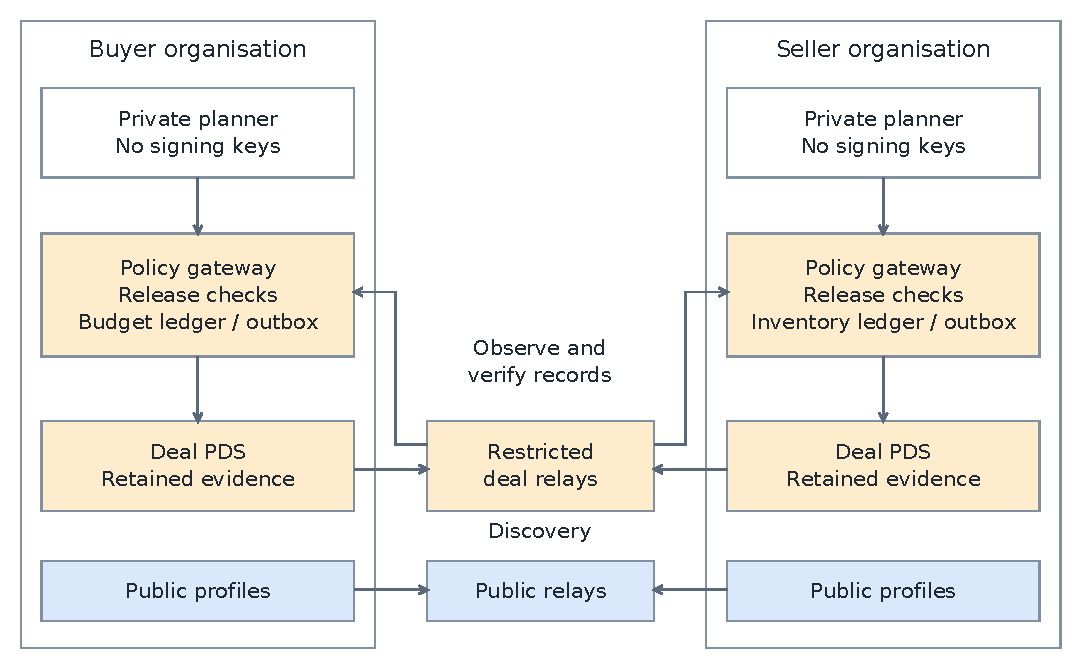
\includegraphics[width=\textwidth]{figures/talea-a2b-deployment.pdf}
\caption{Proposed Talea deployment for A2B. Private planners submit actions to organisational policy gateways. Approved decisions are committed to local resource ledgers and outboxes before publication to the restricted deal channel. Each party observes and verifies the published evidence. Public profiles support discovery separately. Blue identifies existing protocol components; amber identifies proposed enforcement or restricted deployment arrangements, not implemented confidentiality features of AT Protocol. A2A execution, omitted from this deployment view, uses separately authorised payloads and effect identifiers.}
\label{fig:method-deployment}
\end{figure}

This design assumes trusted gateways, protected signing credentials and durable, serialisable resource ledgers. All writers of the controlled resources must obey the same admission rules. Agents, counterparty messages and agent cards are untrusted. The network may delay, reorder, duplicate or temporarily lose events; processes may crash and recover with durable state intact. Signature forgery and hash collisions are excluded. Eventual recovery and message delivery are required for progress, not for the local safety conditions. Deadlines use the designated decision authority's local clock; record timestamps do not supply a globally trusted time. The mechanism does not prevent an organisation controlling its own gateway from signing false statements or refusing performance. Signed evidence supports attribution, while resource safety depends on the ledger and gateway enforcing the specified rules.

\subsection{From a proposal to a resource-backed commitment}

Consider the accommodation purchase developed in Section~\ref{sec:example}. The airline is the buyer and the hotel is the seller. Their agents may negotiate a block of rooms, but each organisation must separately authorise the resulting obligation. The airline delegates permission to accept qualifying offers within a defined scope and exposure limit; the hotel delegates permission to confirm bookings against its available inventory. A delegation defines what an agent may do. The transaction-specific mandate and retained authority receipt identify the particular acceptance authorised under that delegation. Neither permission nor a signed message establishes that funds or rooms remain available.

Suppose the hotel's revised offer is acceptable to the airline. Before publishing acceptance of that exact version, the airline gateway reserves its maximum financial exposure. The hotel gateway then verifies the acceptance and its authority evidence before allocating rooms and issuing confirmation. If it cannot admit the booking, it closes the revision. These steps connect three distinct facts: the terms the agents selected, the authority under which each organisation acts, and the resources backing the resulting commitment. Figure~\ref{fig:method-evidence} shows these dependencies; the following rules specify their admission and recovery semantics.


A commercial record identifies a deal $d$, a revision $v$ and a versioned domain profile. An offer $o$ fixes the parties, quantities, units, currency, price, conditional charges, cancellation terms, framework-agreement reference and seller decision deadline. Monetary amounts use integer minor units. The profile defines rounding and the maximum exposure $E(o)$; autonomous acceptance is refused when that exposure cannot be bounded. A revised offer is a new record. Assessments and acceptances identify the exact offer version, so a check performed on earlier terms cannot silently authorise revised terms.

The proposed sequence is offer--accept--confirm. Acceptance reserves the buyer's maximum exposure; confirmation allocates the seller's inventory. Let $B$ denote the buyer's budget, $C$ its committed exposure and $R$ its outstanding reservations. For inventory class $k$, let $I_k$ denote available total capacity, $A_k$ existing allocations and $q_k(o)$ the offered quantity. Admission requires
\begin{align}
C+\sum_{r\in R}E(r)+E(o)&\leq B,
\label{eq:method-budget}\\
A_k+q_k(o)&\leq I_k\quad\text{for every }k.
\label{eq:method-stock}
\end{align}
The checks and updates must share a local serialisation boundary. Checking a balance and reserving it later would allow concurrent acceptances to spend the same funds. The buyer therefore writes the reservation, accepted offer reference, authorisation evidence and publication-outbox entry in one transaction. A uniqueness constraint on organisation, deal, revision and action prevents a repeated proposal from creating another reservation.

The seller verifies the offer reference and buyer authority evidence, then checks its own authority and inventory. In one transaction it writes exactly one terminal decision for $(d,v)$: confirmation with inventory allocation, or closure. Closure prohibits a later confirmation of that revision. The transaction must control the actual resource ledger, or use a reservation API with equivalent semantics. A separate gateway database cannot ensure inventory safety if other systems can allocate that inventory independently.

Let $a$ be an acceptance and $c$ a confirmation. Observable commitment evidence is
\begin{equation}
\begin{aligned}
\mathrm{Committed}(d,v)\iff{}&\mathrm{Valid}(o,a,c)\\
 &\land\ a.\mathrm{offer}=(\mathrm{URI}(o),\mathrm{CID}(o))\\
 &\land\ c.\mathrm{accept}=(\mathrm{URI}(a),\mathrm{CID}(a)),
\end{aligned}
\label{eq:method-commit}
\end{equation}
where $\mathrm{Valid}$ requires authenticated records, matching deal, revision, parties and profile, and the required authority evidence. This predicate specifies what a verifier inspects; it does not prove that a dishonest gateway reserved resources. The parties' framework agreement determines legal effect.

Figure~\ref{fig:method-evidence} specifies the evidence structure for an admitted commitment. Whereas Figure~\ref{fig:a2b-evidence-gap} asks whether the required connections exist, this graph identifies exact offer and acceptance references, authority evidence, and the local ledger writes required by the method. It represents dependencies, not message order.

\begin{figure}[htbp]
\centering
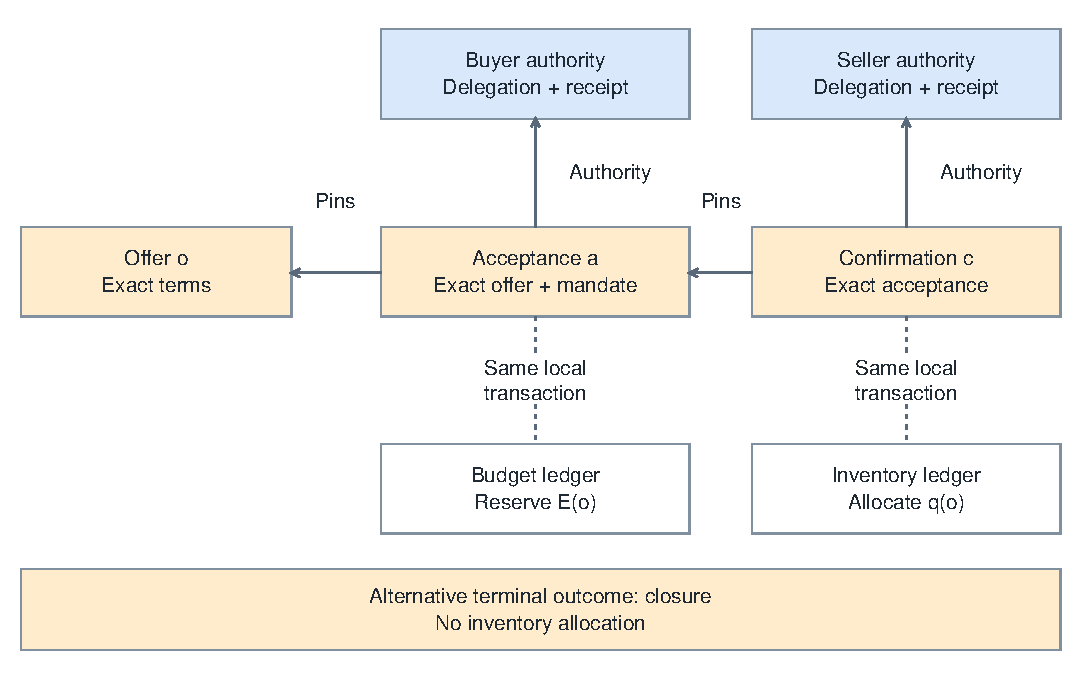
\includegraphics[width=\textwidth]{figures/talea-commitment-evidence.pdf}
\caption{Evidence and resource backing for one commitment. Horizontal arrows labelled ``Pins point from a citing record to its exact referenced content, identified by URI and CID. Amber denotes commercial records, blue denotes authority evidence and white denotes resource ledgers. Vertical arrows identify required authority evidence. Dashed links pair acceptance with buyer reservation and confirmation with seller allocation in their respective local transactions. Authority receipts are assertions by trusted gateways, not proofs of honest accounting. Closure is an alternative terminal decision for the same revision; it allocates no inventory and permits release only after verification. These links express the proposed method, not a global atomic transaction.}
\label{fig:method-evidence}
\end{figure}

\begin{algorithm}[t]
\caption{Gateway admission, publication and buyer reconciliation}
\label{alg:method-admission}
\KwIn{authenticated caller, action, offer $o$, deal revision $(d,v)$}
\KwState{authoritative policy and resource ledgers; durable action and terminal slots; buyer state; publication outbox}
\textbf{Admission at the acting organisation}\;
Resolve the caller's permitted signer; reject identity mismatch or malformed references\;
Begin a serialisable local transaction\;
\If{this action already has a durable outcome}{return the stored outcome without another resource update\;}
Verify the profile, exact terms, action authority and permitted release\;
\uIf{action is acceptance}{
Reject if buyer state is closed or committed\;
Check Eq.~\ref{eq:method-budget}; reject if admission fails\;
Reserve $E(o)$; set buyer state to reserved; store acceptance and authority receipt\;
}
\uElseIf{action is confirmation}{
Verify acceptance, exact offer binding and buyer authority evidence\;
\If{a seller terminal decision already exists}{return that decision\;}
\uIf{deadline permits confirmation and Eq.~\ref{eq:method-stock} holds}{
Allocate inventory; store confirmation in the terminal slot\;
}\Else{store closure in the terminal slot\;}
}
\uElseIf{action is closure}{
\If{a seller terminal decision already exists}{return that decision\;}
Store closure in the terminal slot; allocate no inventory\;
}\Else{abort and reject\;}
Store exact publication bytes and a stable record key in the outbox; commit\;
\textbf{Publication worker:} publish stored bytes; on retry, verify existing content at the same key; escalate conflicts\;
\BlankLine
\textbf{On receipt of a seller terminal record at the buyer}\;
Verify signer, deal, revision and required reference bindings\;
Begin a serialisable local transaction\;
\If{this terminal outcome is already applied}{return without accounting changes\;}
\uIf{record confirms and buyer state is reserved}{
Atomically move $E(o)$ from reserved to committed exposure; set state to committed\;
}
\uElseIf{record closes and buyer state is unseen or reserved}{
Release any reservation; set state to closed, preventing later acceptance\;
}\Else{retain current accounting; quarantine the inconsistent outcome\;}
For a consistent outcome, persist its reconciliation marker with the state change; commit\;
\textbf{Timeout:} retain reservation and query the terminal outcome; silence releases no funds\;
\end{algorithm}

The buyer retains its reservation until it learns the terminal outcome. Passing the seller's decision deadline does not establish closure: a confirmation may already exist but be delayed in transit. The seller may close an undecided revision after expiry, but the buyer releases funds only after verifying the seller's closure for that revision. A recovery service may retrieve this evidence; independent third-party cancellation or release is outside the specified protocol. This choice preserves backing for an unresolved obligation at the cost of blocking during a partition~\citep{graylamport2006}. Superseding an offer likewise cannot cancel an acceptance already in transit without resolving its original revision.

\subsection{Safety properties of the initial commitment}

The following propositions concern initial deal revisions with fixed, non-negative exposure. They assume authenticated records, trusted gateways, durable serialisable ledgers, and enforcement by every writer of the controlled resources. Budget $B$ is fixed during the trace. Each revision has one durable buyer state, either unseen, reserved, committed or closed. Reconciliation atomically updates this state and its accounting entries. A verified closure received before acceptance records a closed state and prevents subsequent acceptance of that revision; repeated messages do not change an already reconciled state. Amendments, settlement, loss of durable state and third-party cancellation are outside these proofs.

\begin{proposition}[Budget preservation]
\label{prop:budget-safety}
Let $U=C+\sum_{r\in R}E(r)$ denote accounted exposure. If $U\leq B$ initially, and every acceptance is admitted atomically only when $U+E(o)\leq B$, then $U\leq B$ after every transition of the initial-commitment protocol.
\end{proposition}
\begin{proof}
Proceed by induction over the serialised buyer transitions. An admitted acceptance adds $E(o)$ to the reserved exposure only after checking the bound. Confirmation reconciliation removes that amount from reservations and adds the same amount to committed exposure, leaving $U$ unchanged. Closure reconciliation removes a non-negative reservation. A closure recorded before acceptance changes no exposure and prevents later acceptance. Publication, timeout and repeated delivery change neither accounting entry. Each transition therefore preserves the bound, completing the induction.
\end{proof}

\begin{proposition}[Exclusive terminal decision]
\label{prop:terminal-exclusivity}
If the seller admits confirmation or closure only by an atomic transition of the same durable decision slot from undecided to a terminal state, and terminal states are irreversible, then one revision cannot have both an admitted confirmation and an admitted closure.
\end{proposition}
\begin{proof}
Serialisability orders competing attempts on the slot. The first successful transition replaces undecided with one terminal state. Every subsequent attempt observes a terminal state and returns the existing decision without replacing it. Thus the other terminal transition cannot succeed. Publication retries reproduce the stored decision and introduce no additional transition.
\end{proof}

\begin{proposition}[Backing during delayed communication]
\label{prop:reservation-backing}
Suppose the buyer durably reserves $E(o)$ before publishing acceptance, the seller confirms only that exact accepted revision, and the buyer releases the reservation only on verified seller closure. During the initial-commitment lifecycle, every seller-confirmed revision retains its exposure in either the buyer's reservation or its committed accounting entry, despite message delay or duplication.
\end{proposition}
\begin{proof}
Confirmation requires an acceptance whose publication follows durable reservation. By Proposition~\ref{prop:terminal-exclusivity}, a confirmed revision cannot also have a valid seller closure. The buyer therefore cannot take the release transition for that revision. Before confirmation is observed, the reservation remains; after atomic reconciliation, its value is transferred to committed exposure. Timeout and duplicate messages do not alter either conclusion. Backing is preserved, although an unavailable terminal record can prevent progress indefinitely.
\end{proof}

These are conditional invariants of familiar transaction mechanisms, not new guarantees supplied by AT Protocol. A gateway implementation must enforce the assumed transitions, and the finite checks in Section~\ref{sec:research-agenda} cover only their stated abstraction. Testing H1 additionally requires varying the coordination design while holding these controls constant.

\subsection{Recovering decisions and controlling disclosure}

Local resource decisions and remote publication are separate operations. A durable outbox stores exact record bytes and a deterministic record key in the decision transaction. Publication retries reuse both. After a crash between publication and acknowledgement, the worker reads that key and compares its content identifier; a conflicting value requires investigation rather than a second decision. Each party retains the offer, acceptance, terminal record, repository inclusion evidence, trusted historical identity material and authority receipts. An AppView cursor cannot replace this evidence or the resource ledger.

Externally effective fulfilment or payment is authorised from durable confirmed state and carries an operation identifier containing the deal, revision and action. Downstream systems must suppress duplicates or expose an identifier that permits reconciliation. A2A task identifiers and repository replication alone do not establish exactly-once effects. Amendments refer to an existing commitment and require a new confirmed revision; fulfilment and settlement remain distinct from commitment.

For multi-party operation, Talea requires ownership-gated dispatch: each bridge acts only for agents operated by its organisation, although several bridges may observe the same public mention. This rule is proposed, not implemented in the sandbox, and does not by itself prevent duplicate dispatch by replicas within one organisation. Bridge high availability therefore requires a separate deduplication mechanism. For participants publishing at both public and private levels, the design uses a separate identity at each level. An approved public sub-request starts a new public thread rather than referencing its private parent; the orchestrator retains the correlation privately. Reconstruction is consequently limited by each participant's authorised view, rather than exposing a complete cross-level history.

Commercial records are exchanged through a restricted deal channel. Access enforcement must cover record reads, exports, blobs, relay streams and derived indexes, rather than only relay crawl selection. A counterparty authorised to read an offer is not necessarily authorised to read the private information used to construct it. We therefore separate a private planner from an outbound emissary and place a deterministic release interface between them, following the distinction between access and declassification~\citep{myers1997,robustdecl}. Neither agent holds unrestricted commercial signing authority.

For private state $P$, approved work order $u$, recipient $q$ and release policy $\pi$, the outbound message is
\begin{equation}
m=\mathrm{Encode}_{p}\bigl(D_{\pi}(P,u,q),\mathrm{PublicContext}\bigr),
\label{eq:method-release}
\end{equation}
where $D_{\pi}$ constructs the permitted values and $p$ is the agreed message profile. The work order fixes the projection, recipient and invocation identifier. The gateway checks field domains and call quotas; the planner cannot replace values with free-form text derived from private context. A field allowlist alone would leave an encoding channel through the agent's choice of permitted values. For procurement, an approved release may disclose the required part, quantity and delivery date while withholding the buyer's maximum budget. Unrestricted adaptive negotiation needs additional release rules; timing and inference across multiple interactions remain outside this limited disclosure guarantee. If the information needed to perform a task cannot be released under the policy, the task must be executed privately or declined. Separating planner and emissary does not make the arguments passed between them safe: those arguments remain the declassification boundary. Publication may leave copies beyond the author's control, so deletion cannot substitute for checking release before publication.

\subsection{Execution options and evidence boundary}

Agent Substrate is a possible runtime for the A2A services, rather than a replacement for the coordination record. A proposed adapter would map an authenticated agent identity to a Substrate actor and route the task through its ingress for resumption and execution~\citep{substrateoverview,substratearchitecture}. Signing, resource accounting and operation identifiers must remain outside rollback-prone actor snapshots, and resumed execution must reconcile with the current durable decision. Authentication, timeout, cancellation and retry behaviour require integration tests; no combined deployment is reported here.

\begin{table}[htbp]
\centering\small
\caption{Evidence boundary: sandbox coordination versus proposed commercial enforcement.}
\label{tab:method-status}
\begin{tabularx}{\textwidth}{@{}P{3.2cm}LL@{}}
\toprule
Capability & Evidence or status & Remaining validation \\
\midrule
Published routing and A2A dispatch & Sandbox implementation and documented example & Independent organisational deployment \\
Thread reconstruction & History retrieval code; author-reported restart exercise & Missing, delayed and conflicting evidence \\
Multi-party dispatch and privacy topology & Design exercise; not implemented & Ownership enforcement, replica deduplication and private correlation \\
Publication identity & Credential selection in bridge handlers & Authenticated caller-to-signer enforcement \\
Authority and reservations & Proposed gateway and transaction rules & Concurrency, crashes and real resource APIs \\
Controlled disclosure & Proposed work-order release interface & Adversarial content and residual channels \\
Substrate execution & Proposed adapter & Resume, retries and external-effect reconciliation \\
\bottomrule
\end{tabularx}
\end{table}

The method connects three decisions that conversation history alone leaves separate: which terms were accepted, under whose authority, and against which resources. The existing sandbox supplies the published coordination path. The remaining components specify the enforcement and recovery rules needed to use that path for A2B commitments. \Cref{sec:example} runs those rules on a case, first with one counterparty and then with three, to find where the design holds and where it stops.
